\section{倾角影响}
\label{sec:3.2}

本节从计算射线在某些理想条件下的旅行时间来开始地震旅行时间对炮检距依赖关系的
研究。

\subsection{平面反射面情形下的剖面与道集}
\label{sec:3.2.1}

对于反射资料,最简单情况就是如图\ref{fig:ofs/twopoint}所示的一个水平反射分界面。正如所预料的,
零炮检距剖面酷似地层模型。共中心点道集的时距曲线是双曲线,其渐近线是直线,该直线
的斜率等于速度$v_1$的倒数。最基本的数据处理称为共深度点叠加。即CDP叠加。处理中,
将典中心点道集(CMP)的所有记录道进行时差校正,使时距曲线拉平成为直线,然后彼
此相加,所得结果酷似一个零炮检距记录道。所有这些记录道集合起来,就叫作共深度点叠
加剖面。实际上,总是把CDP叠加剖面当作是一个零炮检距剖面来加以解释和进行偏移.
在本节中,我们将要讨论如何避免采用这种流行的、过于简单化的假设。

\begin{figure}[H]
\centering
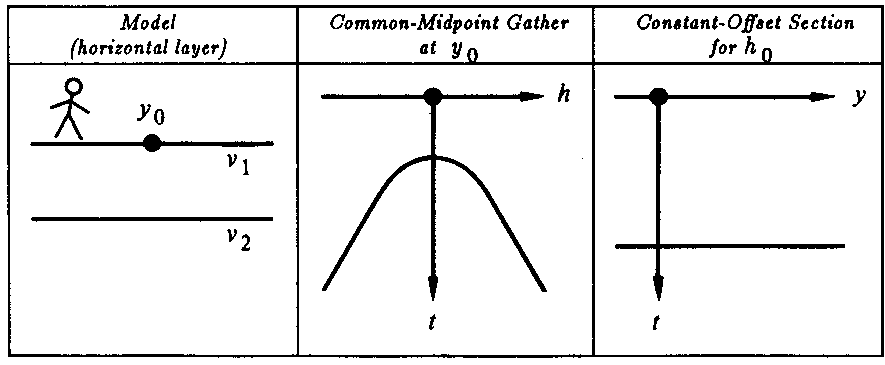
\includegraphics[width=0.65\textwidth]{ofs/simple}
\caption[simple]{最简单的地层模型}
\label{fig:ofs/simple}
\end{figure}

其次一种最简单情形是具有平面反射面,但方向为垂直而非水平。这种情形并不是典型
情形,不过因为地层倾角的影响在极端情形下更易被理解,所以讨论中还是包括了这种情
形。现在,波是沿着空气与大地的分界面传播.为避免混乱,可令反射面以很小的角度偏离
垂直方向,如图\ref{fig:ofs/vertlay}所示。

\begin{figure}[H]
\centering
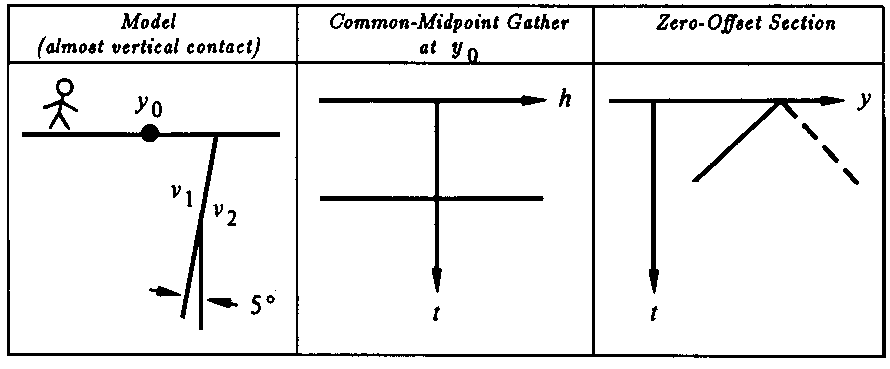
\includegraphics[width=0.65\textwidth]{ofs/vertlay}
\caption[vertlay]{将近垂直的反射面以及相应的道集和剖面}
\label{fig:ofs/vertlay}
\end{figure}

图\ref{fig:ofs/vertlay}表明,旅行时间并不随炮检距之改变而变化。当炮点与检波点彼此逐渐分离
时,旅行时间并不随之增加,看起来似乎有些自相矛盾,解释这种矛盾的关键就在于:保
持恒定不变的是中心点,而不是炮点。在炮检距增大时,炮点虽越易远离该反射面而检波点
却更接近于该反射面,因而,在一个射线路程上的时间减小了,在另一个路程上的时间却增
大了。

平面反射面可以具有位于水平与垂直之间的任何倾角,从而其共中心点道集应处于图
\ref{fig:ofs/twopoint}所示共中心点道集与图\ref{fig:ofs/vertlay}那种共中心点道集之间。
图\ref{fig:ofs/vertlay}内的零炮检距剖面是一条直线,原来它就是双曲线族的渐近线,该渐近线的斜率就等于速度$v_1$的倒数。

\subsection{倾斜层}
\label{sec:3.2.2}

尽管倾斜层形成的时距曲线很简单,要导出它可并不简单。在导出之前,将先说明一下其
结果:对于一个与水平方向呈$\alpha$角度倾斜的地层,其时距曲线为
\begin{equation}
t^2v^2=4(y-y_0)^2sin^2\alpha+4h^2cos^2\alpha
\label{eq:ex3.2.1}
\end{equation}
在$\alpha=45°$情形下,方程\ref{eq:ex3.2.1}是熟悉的毕达哥拉斯(Pythagoras )锥面,它正好像是
$t^2=z^2+x^2$。对于其他的$\alpha$值,该方程仍然是某种锥面,不过是不大熟悉的一种锥面,因为
轴拉长了。

对于$(h,t)$空间内在$y=y_1$点上的共中心点道集,方程\ref{eq:ex3.2.1}看起来如像$t^2=t_0^2+4h^2/v_{apparent}^2$
。所以,不论地层的倾角$\alpha$如何,共中心点道集总是相当于一种严格的双曲线的。倾
角的影响表现在使双曲线之渐近线改变,从而也就是改变着视速度。这个结论在实际工作中
有着重大意义,并以Levin倾角校正而知名(1971 ):
\begin{equation}
v_{apparent}=v_{earth}/cos(\alpha)
\label{eq:ex3.2.2}
\end{equation}
总而言之,倾角使叠加速度増大了。

图\ref{fig:ofs/dipray}表示共中心点道集的若干射线。注意,各条射线是在不同的地点入射在倾斜地
层上。所以,共中心点道集并不就是共深度点道集。要理解为何反射点在反射面上出现移
动,就得回想一下一项基本几何事实,即三角形中的角平分线一般是并不平分对边的。随着
炮检距增大,反射点就向上倾方向移动。

\begin{figure}[H]
\centering
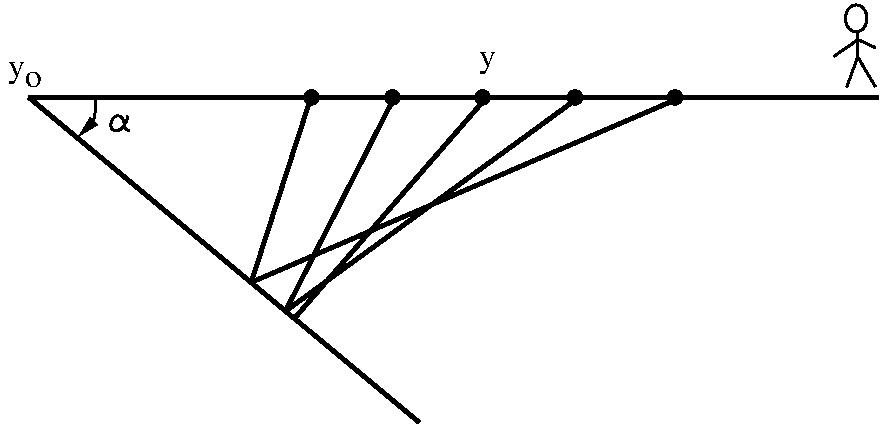
\includegraphics[width=0.65\textwidth]{ofs/dipray}
\caption[dipray]{共中心点道集的射线}
\label{fig:ofs/dipray}
\end{figure}

最后,证明一下式\ref{eq:ex3.2.1}。图\ref{fig:ofs/lawcos}表示的是与位于两倍倾角的另一反射面上的
“虚”震源有关的基本几何关系;为求方便起见,令地层与地面在点相交。根据三角
学的余弦定律可决定图\ref{fig:ofs/lawcos}中的直线之长度为
\begin{figure}[H]
\centering
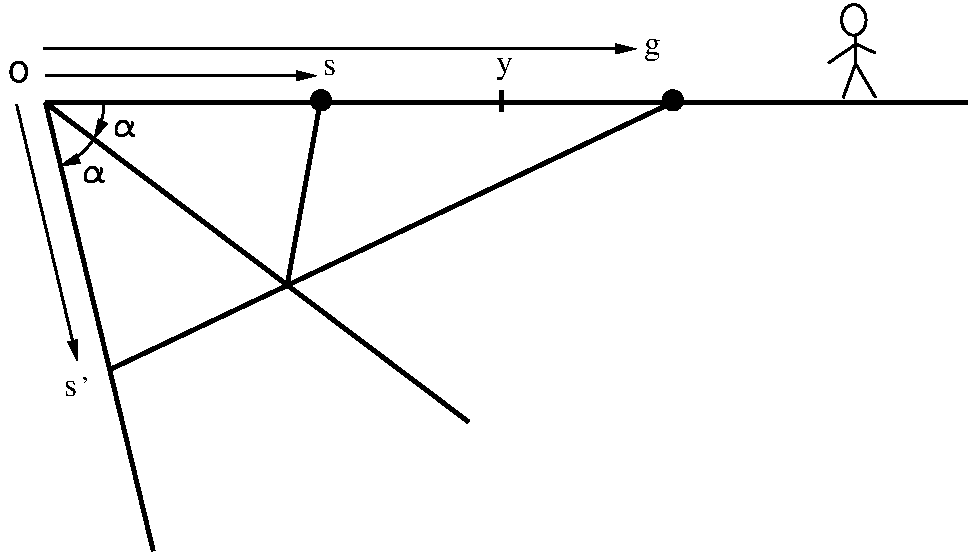
\includegraphics[width=0.65\textwidth]{ofs/lawcos}
\caption[lawcos]{由s'点处之虚震源至g点的旅行时间可用余弦定律表示}
\label{fig:ofs/lawcos}
\end{figure}
\begin{gather*}
t^2v^2=s^2+g^2-2sgcos2\alpha
t^2v^2=(y-h)^2+(y+h)^2-2(y-h)(y+h)cos2\alpha
t^2v^2=2(y^2+h^2)-2(y^2-h^2)(cos^2\alpha-sin^2\alpha)
t^2v^2=4y^2sin^2\alpha+4h^2cos^2\alpha
\end{gather*}
上式就是方程\ref{eq:ex3.2.1}。

式\ref{eq:ex3.2.1}的另一层意思就是:它所描述的是恒定炮检距剖面。出人意外,一个倾斜
的平面地层的旅行时间关系竟在非零炮检距上变得很弯曲——它变成太过分的双曲线了。

\subsection{点源响应}
\label{sec:3.2.3}

另一种简单几何关系是一个反射点位于地层之内时的情形。一个波从任何方向入射在该
点上,将沿所有的方向发生波的反射,由于任何模型都是这类点散射的一种叠加结果,所以这
种几何关系特别重要。图\ref{fig:ofs/twopoint}所示是一个例子。该图中的曲线包括有平点(flat spots),以
这种现象同图\ref{fig:ofs/simple}和图\ref{fig:ofs/vertlay}中的某些曲线呈直线形式是出于相同的原因。
\begin{figure}[H]
\centering
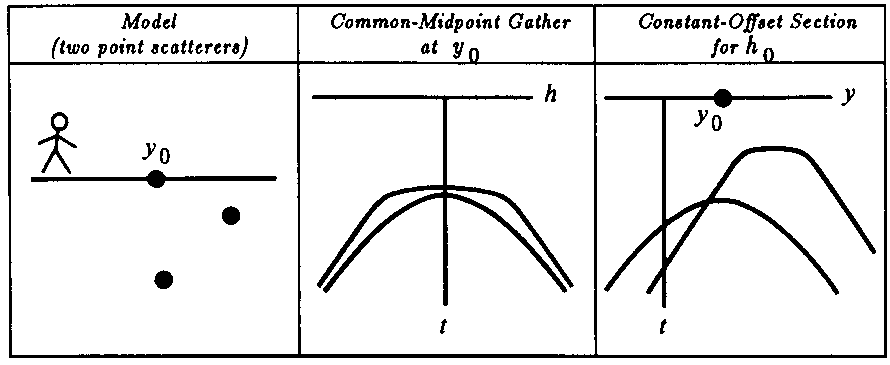
\includegraphics[width=0.65\textwidth]{ofs/twopoint}
\caption[twopoint]{两个点散射之响应。注意图中的平点}
\label{fig:ofs/twopoint}
\end{figure}
一个位于$(x,z)$点上的点散射之几何关系,如图\ref{fig:ofs/pgeometry}所示。
\begin{figure}[H]
\centering
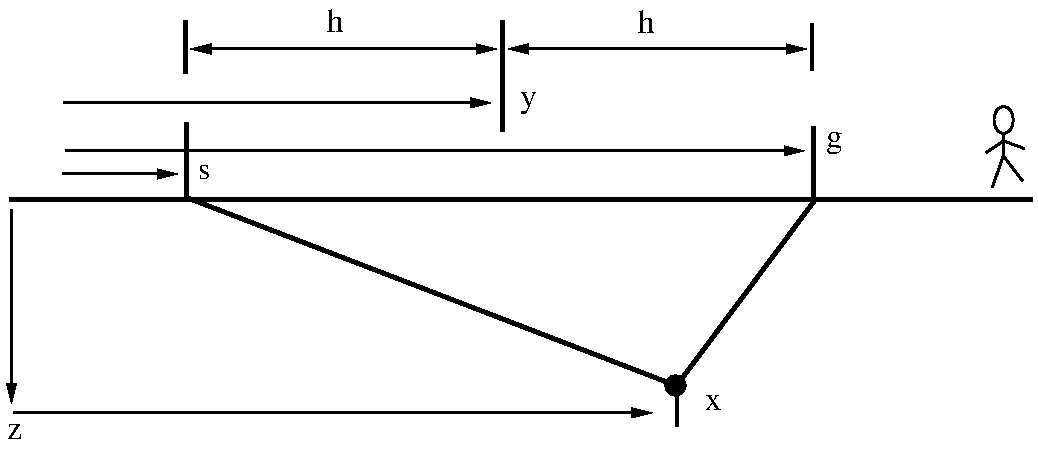
\includegraphics[width=0.65\textwidth]{ofs/pgeometry}
\caption[pgeometry]{点散射几何关系}
\label{fig:ofs/pgeometry}
\end{figure}
旅行时间$t$的方程就是两个旅行路程之和
\begin{equation}
tv=\sqrt{z^2+(s-x)^2}+\sqrt{z^2+(g-x)^2}
\label{eq:ex3.2.3}
\end{equation}

\subsection{Cheops金字塔}
\label{sec:3.2.4}

由于点散射模型之重要性,我们将求助于各种长度关系,以便使式\ref{eq:ex3.2.3}中的$t$、$z$、
$x$、$s$与$g$之间的函数关系具体可见。利用一维图形来表示这种反映爆炸反射面几何形态的圆
锥曲线剖面是非常困难的。

首先,假设式\ref{eq:ex3.2.3}中的第一个平方根式是常数,因为现在令其中任何项均保持为
常数。这样,就剩下$(g,t)$空间内熟悉的双曲线了,除了对时间已经加上一个常数以外。
相反,再假设另一项平方根值为常数,类似地由此又得出$(s,t)$空间内的一个双曲线。在
$(s,g)$空间内,旅行时间等于$s$的一个函数加上$g$的一个函数。我想,这图像有点像是一个
平行于$s$轴的衣架,同另一个平行于J轴的衣架柑交地悬挂着。

旅行时间与各坐标的关系图形犹如是耸立在$(s,g)$平面上或者$(y,h)$平面上的一座山。如
图\ref{fig:ofs/cheop}(a)所示。注意,在大$t$时通过该山的一个横切面是方形的,方形的各角已经加以平
滑。 一个恒定的$t$值就相应于$(s,g)$空间内的一个方形等高线,如图\ref{fig:ofs/cheop}(b)所示。从代
数上说,在一个点反射体接近于地表面的情形下,例如当$z\rightarrow 0$时,该种方形的性质就变得更
为明显,这时,式\ref{eq:ex3.2.3}变为
\begin{equation}
vt=\mid s-x \mid + \mid g-x\mid
\label{eq:ex3.2.4}
\end{equation}
该正方形之中心位于$(s,g)=(x,x)$。令旅行时间$t$沿垂直于$(s,g)$空间内的水平面的
方向向下增大,则相应的方形等高线形状看起来就像是通过埃及Cheops金字塔的一个水平切片
一般。在一定高度环绕该金字塔走一圈,就是环绕方形走一圈。从另一种角度看,在
$s$为恒定的情形下,沿$g$方向横穿过该金字塔时的高度变化,简单就是一个常数加上一个绝对
值函数,保持恒定而沿$s$方向横穿过时的情形也是一样。
\begin{figure}[H]
\centering
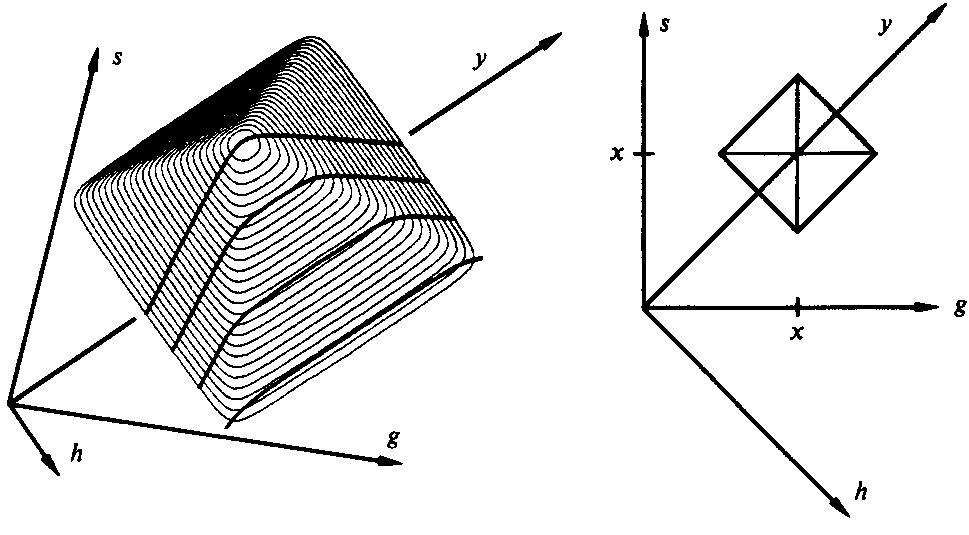
\includegraphics[width=0.65\textwidth]{ofs/cheop}
\caption[cheop]{(a)图为方程\ref{eq:ex3.2.3}在$x$和$z$固定时的旅行时间图像,
看起来像一座山,其中,粗黑线是恒定炮检距剖面。(b)图
为大$t$时(或小$z$时)通过该山的一个横断面}
\label{fig:ofs/cheop}
\end{figure}
更为有趣但不显而易见的情形是共中心点道集的各种曲线和恒定炮检距剖面。回想一
下,根据定义,位于炮点与检波点之间的中心点其坐标为力$y$;再有,$h$等于从炮点至检波点
的水平偏移距离的二分之一
\begin{subequations}
\begin{equation}
y=\frac{g+s}{2}
\label{eq:ex3.2.5a}
\end{equation}
\begin{equation}
h=\frac{g-s}{2}
\label{eq:ex3.2.5b}
\end{equation}
\label{eq:ex3.2.5}
\end{subequations}
$h$恒定时,沿$y$方向的横截面如图\ref{fig:ofs/cheop}所示。在该横截面的最高处,你是在一个如图\ref{fig:ofs/twopoint}秃
顶双曲面的平坦水平阶地上行走。金字塔的顶部和各凌角经受某种侵蚀而被平滑后,就很像
是非零反射面深度情形下的这么一种模型。

在各射线均接近于垂直的情形下,时距曲线均远离双曲线之渐近线,这时式\ref{eq:ex3.2.3}
中的各平方根均可按Taylor级数展开,近似代表一个旋转拋物面,金字塔受侵蚀的顶部形
状可用此描述。

\subsection{随机分布的点散射}
\label{sec:3.2.5}

图\ref{fig:ofs/randcos}所示是取自大约包含有五十个随机分布点散射体所形成之地层模型的一个合成
共炮检距时间剖面(COS),其中到达时间较晚者呈双曲线形,早到达者则双曲线具有平坦的
顶部。最早到达的可能初至相应于射线水平地从炮点直接到达检波点。
\begin{figure}[H]
\centering
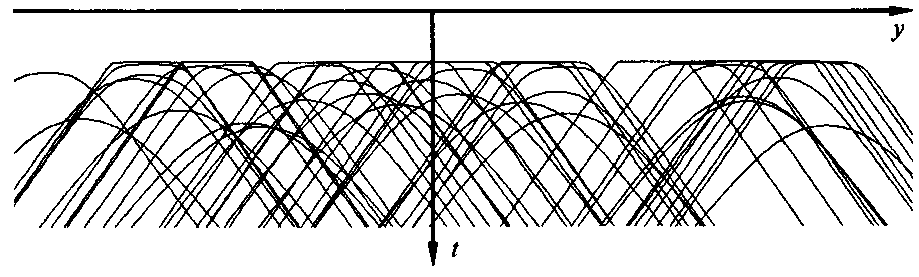
\includegraphics[width=0.65\textwidth]{ofs/randcos}
\caption[randcos]{随机分布点散射体形成的共炮检距时间剖面}
\label{fig:ofs/randcos}
\end{figure}

图\ref{fig:ofs/randcsp}所示是由同一个随机分布点散射的地层模型作出的合成共炮点剖面(CSP)。
其中,每个散射体均形成一个S曲线型的时距曲线。在零炮检距附近,各双曲线均不对称,
它们的位置是随机的,不过,它们必然全都位于各直线$\mid g-s\mid=vt$之下。不但在较早的时间
上,而且在较晚的时间上,都可以发现具有尖锐顶部的双曲线。然而,由检波点附近的浅层
散射侔所形成的各尖锐顶部必然都位于接近于各直线$\mid g-s\mid=vt$之处。

\begin{figure}[H]
\centering
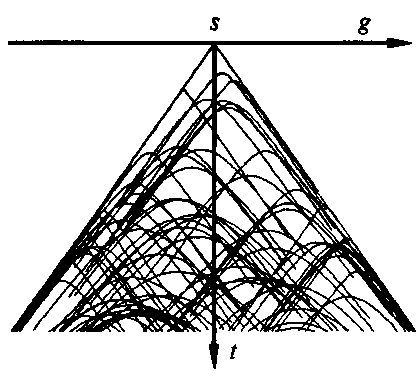
\includegraphics[width=0.65\textwidth]{ofs/randcsp}
\caption[randcsp]{随机分布点散射体形成的共炮点剖面}
\label{fig:ofs/randcsp}
\end{figure}

图\ref{fig:ofs/randcmp}的左图所示是由包含有大约五十个随机分
布点散射体的一个地层模型所形成的合成共中心点道集
(CMP)。因为这是一种共中心点道集,各曲线经过零
炮检距时均呈对称(野外资料的各负值炮检距从不绘
岀)。某些双曲线具有平坦的顶部,这表明相应散射点均非直接位于中心点之下。

\begin{figure}[H]
\centering
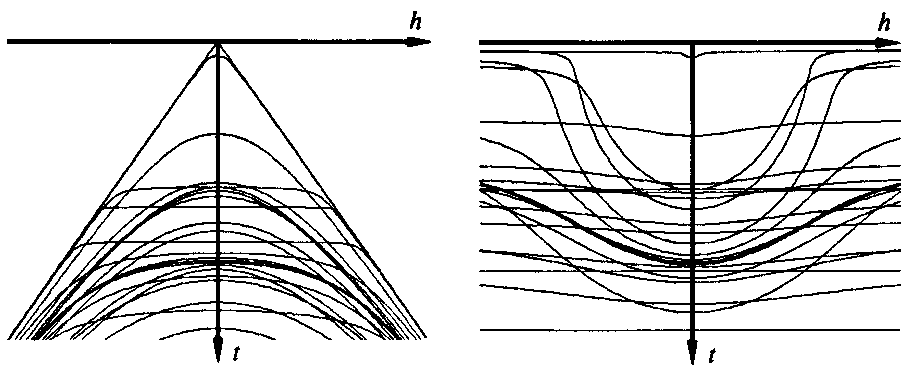
\includegraphics[width=0.65\textwidth]{ofs/randcmp}
\caption[randcmp]{随机分布点散射体形成的共中心点道集(左图)。同一
道集经过时差校正之后的情形(右图)}
\label{fig:ofs/randcmp}
\end{figure}

正常时差校正是对数据资料进行拉伸处理,试图使
馭曲线变成平缓,这种校正要求地层要平坦,但是对于
直接位于中心点之下的点散射体,这种处理也是有效
的。图\ref{fig:ofs/randcmp}的右图表示对随机散射体模型应用正常
时差校正时会发生什么现象,这时某些反射被展平了,另外一些则“过校正”了。 

\subsection{正向与反向散射:Larner条痕}
\label{sec:3.2.6}

在某些地段上,远地表波(near-surface wave)压制了有地质意义的深层反射。由于
地表面比起下面较深地层更为大大地不规则,所以近地表波通常均不规则,这使得我们的困
难复杂化了。在陆地上,这些干涉波称作地滚波;在海上,它们称作水波(water wave),
但别把它们与水面上的表面波相混。

图\ref{fig:ofs/vertlay}中垂直的反射壁就可能是产生这类近地表干扰的一种模型,在这种模型中,波
仍然是靠近地表传播的。随机分布的垂直壁可以形成类似图\ref{fig:ofs/shelikof}所示野外资料那样的零炮
检距时间剖面。另一类不太少见的近地表干扰模型就是随机点散射模型中的平顶曲线了。

\begin{figure}[H]
\centering
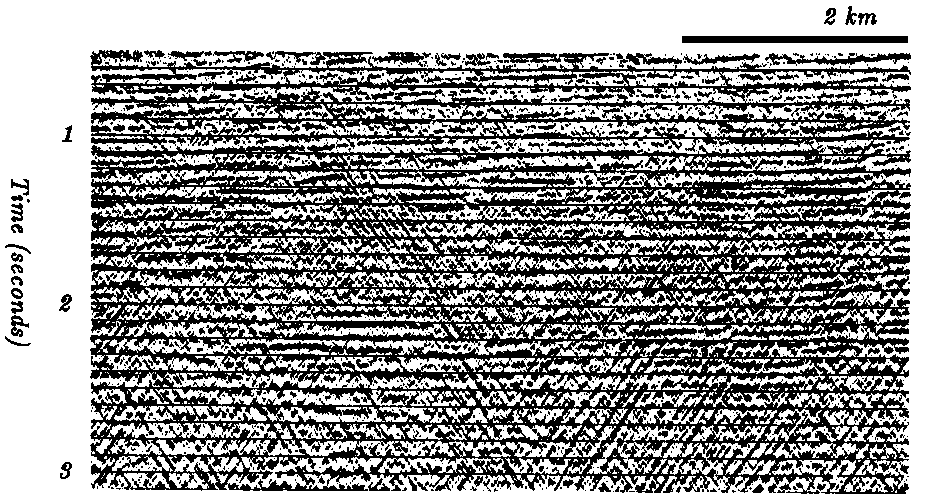
\includegraphics[width=0.65\textwidth]{ofs/shelikof}
\caption[shelikof]{阿拉斯加地区Slielikof海峡的具有水层干扰之共深度点迭加时间剖面(据Lamer
) }
\label{fig:ofs/shelikof}
\end{figure}

在随机点散射模型中,速度是一项常数。在实际情况下,对近地表波来说,地层速度一
般比较低,对深层反射来说,速度一般比较高,这就使放大某种不受欢迎的干扰有了可乘之
机。

进行共深度点叠加可使具有叠加速度的同相轴得到加强,压制具有其他速度的同相轴。
因而你也许会猜想,在较深部位上进行叠加,较高的速度将会压制具有低速度的近地表同相
轴。其实大谬不然,近地表干扰都不是从水平地层发生反射;它们倒是非常像是从垂直壁或陡
倾斜地层发生的反射,式\ref{eq:ex3.2.2}指出,倾角增大将使视速度増加,所以,毫不奇怪,在深
层地层上进行叠加时,高速度可能使地表干扰加强。Larner等人(1981
)已经清楚地描述和解释过实际工作中出现的这种现象。

\subsection{侧反射的速度}
\label{sec:3.2.7}

浅水干扰可能由沉没船只的散射波所形成,或者是距测线若干公里之遥的某个岛屿或冰
山的侧面所散射的波。想一想散布在整个浅海海底的漂砾吧,它们不但沿着船的航道分布,
而且沿其两側散布。由这些漂砾形成的反射时距曲线正好适甩随机点散射模型。由于地震波
具有较长的波长,接收设备使我们无法将这些侧反射与上、下行波加以区别。

试想像位于船的一侧有若干公里之遥的这些浅层散射体之一,更准确地说,应令该散射
体处于海底表面上,位于垂直通过炮点与检波点连线的中点之直线上。对于这一个散射体来
说,其共中心点道集应是一精确的双曲线,犹如是图\ref{fig:ofs/randcsp}上之深层反射体所形成的一般,
既然这是一个由水层速度决定其形态的双曲线,以沉积地层较高的速度进行的共深度点叠加
方法应当能很好地压制掉这类散射干扰。所以,以前述及的产生“坑蓆状干扰”\footnote{Larner Streaks}的散射不是侧
向散射,“坑蓆状干扰”的散射是由那些沿着测线分布的散射体所形成,而不是由垂直于测
线方向分布的散射体所形成。

\subsection{偏移椭圆}
\label{sec:3.2.8}

另一种深刻了解方程\ref{eq:ex3.2.3}的办法是把炮检距$h$和总旅行时间$t$看作固定常数,这时
最终可证明,可能的反射点的轨迹在$(y-y_0,z)$平面上应是一个椭圆。之所以为椭圆的
原因可由椭圆的几何意义得出。要画出一个椭圆,可将一个钉子或图钉固定在图\ref{fig:ofs/pgeometry}的
$s$处,另一个则钉于$g$处,用一根线将图钉联结起来,线的长度应足以从$s$经$(y_0,z)$至$g$。
用一支铅笔沿该线滑动同时保持该线是绷紧着的,那就可以作出一个经过
$(y_0,z)$点的椭圆了,该线应使总距离化保持为常数。

